\documentclass[11pt]{article}
\usepackage[margin=1in]{geometry}
\usepackage[utf8]{inputenc}
\usepackage[T1]{fontenc}
\usepackage{lmodern}
\usepackage{microtype}
\usepackage{booktabs}
\usepackage{multirow}
\usepackage{amsmath}
\usepackage{graphicx}
\usepackage{pgfplots}
\pgfplotsset{compat=1.17}
\usepackage[numbers,sort&compress]{natbib}
\usepackage[hidelinks]{hyperref}
\usepackage{xcolor}
\usepackage{caption}
\setlength{\tabcolsep}{4.5pt}
\captionsetup{font=small,labelfont=bf}

\newcommand{\fone}{$f@1$}
\newcommand{\fthree}{$f@3$}
\newcommand{\todo}[1]{\textcolor{red}{[#1]}}

\title{When Routing Benchmarks Reward Repetition:\\
\large Evaluating Recipient Selection in a Persistent Agent Mesh}

\author{Prasanna Ravishankar\\
\small \texttt{me@prassanna.io}
\todo{affiliation; co-author line}}

\date{Draft of 14 October 2026}

\begin{document}
\maketitle

\begin{abstract}
Routing requests to persistent agents mixes two kinds of decision: repeated contact with the agent the sender spoke to last, and changes of recipient. Aggregate agreement scores merge them. We introduce a history-conditioned evaluation protocol and apply it to an event-journal reconstruction of a production agent mesh. Across 555 worker-directed requests, a small state-informed classifier matches the recorded recipient on 57.8\%, against 60.0\% for a one-line recent-contact rule and 56.0\% for a time-ordered per-sender majority. These totals conceal opposing effects: relative to the majority rule the classifier gains 22 matches on recipient switches, loses 31 on continuations, and gains 19 where the sender has no exchange history. Reweighting the observed conditional scores reverses the ranking without changing either policy. An activity mask, a novelty control and a lexical audit separate residual routing signal from historical cues. The same protocol applied to three frontier models shows where the ceiling is: Claude Opus~5.5 reaches 77.5\% overall and 56.8\% at switches, and when the activity fields are masked it keeps 46.7\% at switches while falling below the habit rule on continuations. The continuation gain of every model is recency read out of the state; the switch gain is the quality of the reading. A DecisionBench replay illustrates why history definitions and label semantics must accompany cross-dataset comparison. We release the reconstruction method, the replay harness and the metric, and derive a frozen, prospectively tested arrival-triggered policy from the error decomposition.
\end{abstract}

\section{Introduction}

A growing class of systems lets language-model agents message one another: a coding agent on one project asks a coding agent on another for a review, an orchestrator dispatches work to whichever peer already holds the relevant worktree, a human relays instructions through a bot. In these systems the recipient of a request is a long-lived peer with a current task, a history with the sender, and a lifetime, not a model drawn from a pool. Today the sender names the recipient. The obvious improvement is to let a model choose, and the obvious way to evaluate the model is to score how often its choice agrees with the recipient the sender would have named.

This paper is about what that score measures. In the mesh we study, two requests in three go to the peer the sender spoke to last. A rule that knows only the sender's previous recipient is right on every one of them and wrong on every other request by construction. A learned router evaluated on the pooled stream is therefore scored mostly on decisions a one-line rule already makes, and its aggregate agreement with the recorded recipient says little about the decisions for which anyone would want a router. Worse, as we show, the aggregate can rank two fixed policies in either order depending only on the proportion of repeated contacts in the evaluation stream.

We make three contributions.

\begin{enumerate}
\item \textbf{A history-conditioned protocol} for evaluating recipient selection among persistent agents. Every request is classified, from information available before it was sent, as a \emph{continuation} (the recorded recipient is the sender's most recent exchange partner), a \emph{switch} (it is not), or \emph{no history} (the sender has no live exchange). Scores are reported per condition, beside analytic chance for the request's candidate set, against temporal baselines that use no future information, with paired tests and an explicit dependence unit.
\item \textbf{An empirical counterexample} drawn from 908 routing decisions reconstructed from a production mesh's event journal, with a replay harness that scores any policy on them. On this data the ranking of a classifier against a habit rule reverses with the request mix; masking every activity-derived field shows what fraction of each model's score is recency; and three frontier models on the same inputs locate the ceiling of state-based routing and show that it, too, is mostly recency on continuations and mostly reading quality at switches.
\item \textbf{A design consequence.} The decomposition shows that the useful work of a router is concentrated on switches and on requests with no history, and that the deployable question is not which recipient to pick but when to override a cheap default. We derive an arrival-triggered override policy, freeze it, and register a prospective test.
\end{enumerate}

We deliberately call the measured quantity \emph{recipient agreement} rather than routing quality. The label is the recipient the sender actually named. It is reproducible and behaviourally meaningful, but it is not a proof that the sender was right, and nothing here measures downstream task outcome.

\section{Setting and the unit of measurement}

\paragraph{The mesh.}
Repowire is a daemon that registers agent peers (coding agents on several backends, a human relay, and job runners) and lets them address one another by name. Peers carry \emph{claimed} state, a free-text self-description, and \emph{attested} state that the daemon observes: backend, project (parsed from the peer's name), liveness and last-seen age, turn activity, open inbound asks, and the time of the peer's last exchange with the sender. We study the period 22 May to 10 August 2026, before the daemon recorded routing snapshots, so claimed state is unavailable and every result below is on attested state only.

\paragraph{The decision.}
A routing decision is a tuple (sender, request text, candidate set with attested state as of the request time, recorded recipient). The candidate set is every peer the daemon would have offered at that moment, excluding the sender and machine identities. A router ranks the candidates; it is scored by whether the recorded recipient is first (\fone) or in the top three (\fthree). A router that declines or fails is scored as a miss and counted as a fallback.

\paragraph{History conditions.}
Let $r$ be the sender's most recent exchange partner at the request time, where an exchange is an ask counted at creation or at its first reply with a message, expiring 24 hours after creation. The request is a \emph{continuation} if the recorded recipient equals $r$, a \emph{switch} if $r$ exists and differs, and \emph{no history} if $r$ does not exist. These conditions use the label and are diagnostics for evaluation, not features a deployed router observes.

\paragraph{Why the mix matters.}
For a policy $\pi$ with conditional agreement $A_{\pi,C}$ on continuations and $A_{\pi,S}$ on switches, agreement on a stream with continuation share $p$ is
\begin{equation}
A_\pi(p) = p\,A_{\pi,C} + (1-p)\,A_{\pi,S}.
\label{eq:mix}
\end{equation}
Two policies with crossing conditional scores are ranked by $p$, which the policy does not control. Section~\ref{sec:decomp} shows that this crossing occurs for every learned router we tested, within the range of mixes seen across real routing datasets.

\section{Reconstruction and protocol}
\label{sec:method}

\paragraph{Reconstruction.}
The daemon's event journal records asks (sender, recipient id, text, time), acks, chat turns, and peer lifecycle events. From these we rebuild each decision's candidate set and attested fields using only events strictly before the request. Liveness is inferred from activity within a 24-hour window, because peer registration events begin after the last ask in the period; candidate sets are therefore a lower bound on the registry and the window is reported as a free parameter. Turn state is the type of the last recorded chat turn within five minutes. Open inbound asks are those not yet closed by an ack or reply. Exchange semantics match the live daemon's tracker event for event; four declared divergences and their per-row impact are listed in Appendix~\ref{app:divergences}.

\paragraph{Population.}
Of 2,545 asks, 1,505 came from machine dispatch and are excluded, with 39 self- or service-addressed. Of the remaining 1,001, the recorded recipient was not observably online for 93 (75 with no prior evidence at all, most of them peers asked at the moment of their spawn). The 908 scorable decisions split into 353 addressed to an orchestrator (which have one answer and are not a routing problem) and 555 addressed to a worker. Table~\ref{tab:population} describes the worker-directed set. Candidate sets have median 12 and mean 16.5 members (max 110). Only 97 of the 555 have an orchestrator as sender; 243 are peer to peer and 215 come through the human relay.

\begin{table}[t]
\centering\footnotesize
\caption{What the evaluation observes. The DecisionBench column is a contrast in history structure (Section~\ref{sec:decisionbench}), not a replication.}
\label{tab:population}
\begin{tabular}{lll}
\toprule
Property & Historical mesh & DecisionBench aware-c2 \\
\midrule
Evaluated decisions & 555 worker-directed, of 908 scorable & 691 delegations \\
History groups & 333 continuation, 169 switch, 53 no history & 93 same, 270 switch, 328 first in task \\
Repeat share, with history & $333/502 = 66.3\%$ & $93/363 = 25.6\%$ \\
Repeat share, all rows & $333/555 = 60.0\%$ & $93/691 = 13.5\%$ \\
Label & Recorded recipient of the ask & Recorded delegate of the orchestrator \\
History semantics & Reconstructed exchanges with expiry & Previous delegation within task \\
Candidate information & Activity-inferred registry, attested metadata & Static model cards \\
\bottomrule
\end{tabular}
\end{table}

\paragraph{Baselines.}
\emph{Recent} picks $r$ and abstains without one. \emph{Newest} picks the candidate with the smallest last-seen age. \emph{Past majority} picks the candidate the sender addressed most often in decisions strictly before this one, and abstains with no vote. \emph{Retrospective majority} votes from the whole window including the future; it is reported only as a leakage reference, never as a deployable arm. \emph{Chance} is the analytic expectation $1/n$ (and $\min(3,n)/n$) of a uniform draw over the row's $n$ candidates, averaged over rows, rather than a seeded draw. \emph{Novelty} picks uniformly among candidates that have never appeared in any prior ask, scored by expectation.

\paragraph{Routers.}
All learned arms receive the same byte-identical attested view of the sender, the request text and every candidate, and return a ranking. \emph{Jev} is a small hosted classifier (TypeSafe) and the instrument of the original study; \emph{Clef Flash} (Cloudflare Workers AI) is a second small hosted ranker; \emph{Claude Haiku~5.5, Sonnet~5.5 and Opus~5.5} are frontier models prompted with the same view under a structured output schema that requires one score per candidate (Appendix~\ref{app:elicitation}). A \emph{claimed} arm sends the classifier the empty description fields only, as a no-information control. The \emph{strict mask} blanks every activity-derived field (last exchange with sender, open inbound asks, last-seen age, turn state) on both the sender block and every candidate, leaving name, project, backend and role.

\paragraph{Inference.}
Rows are paired by decision; differences between arms use exact two-sided sign tests on discordant rows. Because requests share senders and weeks, Section~\ref{sec:dependence} repeats the key tests under sender and week clustering and reports the number of independent blocks. All thresholds examined on this data are labelled exploratory.

\section{Results}

\subsection{The aggregate conceals opposing effects}
\label{sec:decomp}

Table~\ref{tab:decomp} gives the hit counts behind the headline numbers. Over all 555 worker-directed requests the classifier (321 hits) is level with the recent-contact rule (333) and ten hits ahead of past majority (311). Conditioned on history, the same rows show three different stories: on continuations the classifier is 31 hits behind past majority and 96 behind recent contact; on switches it is 22 ahead of past majority and 65 ahead of recent contact, which is zero by definition; on requests with no history it is the only one of the three that answers. Its aggregate edge over the majority rule is entirely the no-history stratum. The switch advantage and the aggregate advantage are different effects.

\begin{table}[t]
\centering\small
\caption{Where aggregate differences come from. Correct matches at rank one, worker-directed requests. Abstentions count as misses.}
\label{tab:decomp}
\begin{tabular}{lrrrrrr}
\toprule
History condition & $n$ & Recent & Past majority & Jev & Jev $-$ majority & Opus 5.5 \\
\midrule
Continuation & 333 & 333 & 268 & 237 & $-31$ & 308 \\
Switch & 169 & 0 & 43 & 65 & $+22$ & 96 \\
No history & 53 & 0 & 0 & 19 & $+19$ & 26 \\
All & 555 & 333 & 311 & 321 & $+10$ & 430 \\
\bottomrule
\end{tabular}
\end{table}

Figure~\ref{fig:mix} plots equation~\ref{eq:mix} with these counts. The classifier crosses past majority at $p = 0.583$ and recent contact at $p = 0.572$; the observed history-bearing mix is $p = 0.663$, so on this stream it loses to both, and on a stream with ten points fewer continuations it would beat both. Nothing about either policy changes between those two readings. The same holds for the frontier models: Haiku and Sonnet cross recent contact at $p = 0.66$, almost exactly the observed mix, and even Opus~5.5, the strongest arm at both ends, falls below the one-line rule once continuations exceed 88\% of history-bearing traffic.

\begin{figure}[t]
\centering
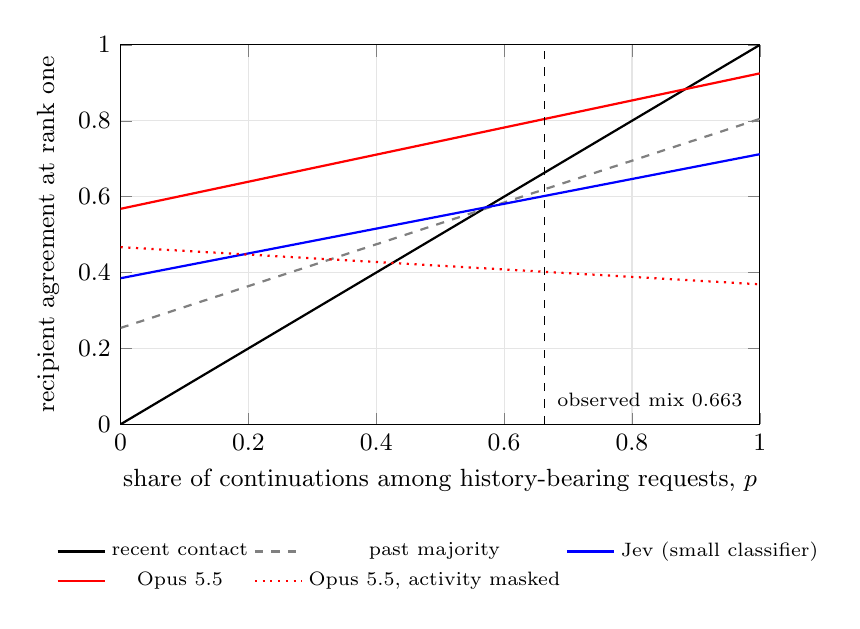
\begin{tikzpicture}
\begin{axis}[
  width=0.8\linewidth, height=6.4cm,
  xlabel={share of continuations among history-bearing requests, $p$},
  ylabel={recipient agreement at rank one},
  xmin=0, xmax=1, ymin=0, ymax=1,
  legend style={font=\scriptsize, draw=none, fill=none, at={(0.5,-0.28)}, anchor=north, legend columns=3},
  grid=major, grid style={gray!20},
  tick label style={font=\small}, label style={font=\small},
]
\addplot[black, thick] coordinates {(0,0) (1,1)};
\addlegendentry{recent contact}
\addplot[gray, thick, dashed] coordinates {(0,0.254) (1,0.805)};
\addlegendentry{past majority}
\addplot[blue, thick] coordinates {(0,0.385) (1,0.712)};
\addlegendentry{Jev (small classifier)}
\addplot[red, thick] coordinates {(0,0.568) (1,0.925)};
\addlegendentry{Opus 5.5}
\addplot[red, thick, dotted] coordinates {(0,0.467) (1,0.369)};
\addlegendentry{Opus 5.5, activity masked}
\addplot[black, dashed, thin] coordinates {(0.663,0) (0.663,1)};
\node[font=\scriptsize, anchor=south west] at (axis cs:0.668,0.02) {observed mix 0.663};
\end{axis}
\end{tikzpicture}
\caption{The winner changes when only the request mix changes. Each line is equation~\ref{eq:mix} drawn through the observed conditional scores in Table~\ref{tab:decomp}. This is a descriptive reweighting of recorded scores, not a forecast under distribution shift; no decision is rerun. Requests with no history are reported separately.}
\label{fig:mix}
\end{figure}

\paragraph{The full ladder.}
Table~\ref{tab:arms} gives every arm on every condition. Three regularities hold across arms. First, on continuations no learned arm beats the recent-contact rule, which scores 1.0 there by construction, and only Opus~5.5 beats past majority. Second, at switches every learned arm beats the temporal baselines that can answer, and chance is an order of magnitude below all of them because candidate sets are largest exactly where the sender is changing recipient (mean 23.3 candidates at switches against 12.3 on continuations). Third, the two small hosted rankers and the two smaller frontier models form a band: Clef Flash is below Jev on every condition, and Haiku and Sonnet are above Jev at switches ($25$--$9$, $p = .009$; $28$--$16$, $p = .10$) but not above the retrospective majority anywhere ($p \ge .14$).

\begin{table}[t]
\centering\footnotesize
\caption{Recipient agreement at rank one by history condition, worker-directed requests. Chance is the analytic uniform expectation. Fallbacks score as misses. Frontier and Clef rows are re-runs on the reconstructed snapshots (October 2026); the retrospective majority uses future votes and is a leakage reference only.}
\label{tab:arms}
\begin{tabular}{lrrrrrr}
\toprule
Arm & All & Contin. & Switch & No hist. & Orch. & Orch. sw. \\
 & 555 & 333 & 169 & 53 & 97 & 62 \\
\midrule
Chance & .134 & .170 & .072 & .109 & .060 & .061 \\
Recent contact & .600 & 1.000 & .000 & .000 & .289 & .000 \\
Newest & .571 & .793 & .195 & .377 & .258 & .048 \\
Past majority & .560 & .805 & .254 & .000 & .454 & .339 \\
Retrospective majority & .658 & .808 & .396 & .547 & .598 & .500 \\
\midrule
Claimed (empty) & .139 & .156 & .095 & .170 & .113 & .129 \\
Clef Flash & .461 & .556 & .314 & .340 & .278 & .290 \\
Jev & .578 & .712 & .385 & .358 & .402 & .371 \\
Jev, strict mask & .312 & .321 & .302 & .283 & .196 & .242 \\
Haiku 5.5 & .631 & .757 & .479 & .321 & .392 & .387 \\
Sonnet 5.5 & .629 & .766 & .456 & .321 & .443 & .403 \\
Opus 5.5 & \textbf{.775} & \textbf{.925} & \textbf{.568} & .491 & .546 & .500 \\
Opus 5.5, strict mask & .389 & .369 & .467 & .264 & .340 & .403 \\
\bottomrule
\end{tabular}
\end{table}

\subsection{Which explanations survive controls}
\label{sec:controls}

A router that agrees with the recorded recipient at switches might be reading the task, or might be reading one of several cheaper cues. We test four.

\paragraph{Activity recency.}
The strict mask removes every field derived from journal activity. For the small classifier it collapses continuation agreement from .712 to .321 and leaves switch agreement at .302, about four times chance and three times the no-information control. For Opus~5.5 it collapses continuation agreement from .925 to .369, below the habit rule, and leaves switch agreement at .467. On continuations, then, nearly the whole score of every model is activity recency read out of the state: the frontier model and the small classifier were both answering ``who did this sender talk to last'' from the fields that encode it. At switches a residual remains that the mask cannot remove, and its size depends on the reader (Section~\ref{sec:frontier}). Two caveats bound this reading: candidate membership is itself activity-selected, so no field ablation removes activity entirely; and the mask also hides the arrival signal a deployed router would see.

\paragraph{Novelty.}
Twenty-nine switches go to a recipient that had never appeared in any prior ask. On those rows a uniform pick among never-asked candidates scores .478 by expectation, above the classifier (.414), the strict classifier (.414) and the newest rule (.276). Given that the target is novel, any novelty rule finds it; the model adds nothing. Across all 169 switches the novelty rule scores .082, so its value is entirely in knowing when to apply it.

\paragraph{Lexical cues.}
Literal recipient addresses (full display name, peer id or handle) appear in 4 of 555 request texts, one of them a switch that every arm misses. Broader project mentions appear in 34\% of switches. On the 111 switches with no detected recipient or project reference, the classifier scores .387 and the strict classifier .342 against past majority .144; on the 58 with a reference, past majority rises to .466 and the strict classifier falls to .224. The strict residual therefore does not depend on the message naming the peer. This establishes robustness to a lexical filter, not semantic understanding.

\paragraph{The dependence unit.}
\label{sec:dependence}
The pooled switch advantage of the classifier over past majority ($46$--$24$, $p = .012$) survives weekly blocking (8 blocks, $p = .031$) but not sender blocking (52 senders, $15$ positive against $7$, $p = .13$; magnitude-weighted sign flip $p = .29$). One sender contributes 16 of the 22 net extra hits; without it the comparison is $49$ against $43$ of 135, $p = .50$. On the 62 switches sent by the orchestrator, which is the population the live system routes, the classifier and past majority are indistinguishable ($14$--$12$, $p = .85$). We therefore report the classifier's switch advantage as nominal and concentrated in one sender's traffic. The frontier result is more robust to the same checks: Opus~5.5 beats past majority on orchestrator switches $17$--$7$ ($p = .064$) and the classifier $13$--$5$ ($p = .096$), and beats both by wide margins pooled (Table~\ref{tab:paired}).

\begin{table}[t]
\centering\small
\caption{Paired comparisons at rank one on the 169 switches (wins--losses on discordant rows, exact two-sided sign test). The right column is the 62 switches with an orchestrator sender.}
\label{tab:paired}
\begin{tabular}{llrlrl}
\toprule
Arm & Against & \multicolumn{2}{l}{All switches} & \multicolumn{2}{l}{Orchestrator switches} \\
\midrule
Jev & past majority & 46--24 & $p=.012$ & 14--12 & $p=.85$ \\
Jev, strict & past majority & 45--37 & $p=.44$ & & \\
Opus 5.5 & retrospective majority & 53--24 & $p=.001$ & 15--15 & $p=1.0$ \\
Opus 5.5 & past majority & 63--10 & $p<10^{-4}$ & 17--7 & $p=.064$ \\
Opus 5.5 & Jev & 38--7 & $p<10^{-4}$ & 13--5 & $p=.096$ \\
Opus 5.5 & Sonnet 5.5 & 24--5 & $p<.001$ & & \\
Opus 5.5 & Opus 5.5, strict & 27--10 & $p=.008$ & & \\
Opus 5.5, strict & retrospective majority & 51--39 & $p=.25$ & & \\
Opus 5.5, strict & past majority & 61--25 & $p<.001$ & 17--13 & $p=.58$ \\
Opus 5.5, strict & Jev, strict & 35--7 & $p<10^{-4}$ & & \\
Opus 5.5, strict & Jev & 31--17 & $p=.060$ & & \\
\bottomrule
\end{tabular}
\end{table}

\subsection{Reading the state well: where the ceiling is}
\label{sec:frontier}

The small classifier was the instrument of the study, not its subject, and a reviewer should ask whether its modest switch residual is a property of the state or of the reader. Running three frontier models on the identical view answers that. Haiku and Sonnet sit with the classifier: a little above it at switches and not above the habit rule anywhere. Opus~5.5 is the first arm that beats the habit rule on every condition where that is measurable: .775 overall against .658 for the retrospective majority ($119$--$54$, $p<10^{-4}$), .925 on continuations ($55$--$16$), .568 at switches ($53$--$24$, $p = .001$), and it does so from attested state alone.

The strict mask then separates what the frontier model reads. Its continuation score falls to .369, below the habit rule, by the same mechanism as the classifier: the gain there was recency. Its switch score falls to .467, which still ties the retrospective majority ($51$--$39$, $p = .25$), beats past majority ($61$--$25$), beats the strict classifier ($35$--$7$, $p<10^{-4}$) and edges the unmasked classifier ($31$--$17$, $p = .06$). Figure~\ref{fig:ladder} lays this out. At switches, agreement decomposes approximately into .30 that any reader extracts from the static state (project, role, backend, name), a further .17 from reading that state well, and about .10 from the activity fields. The static state carries real switch signal that a small classifier does not extract and a frontier model does.

\begin{figure}[t]
\centering
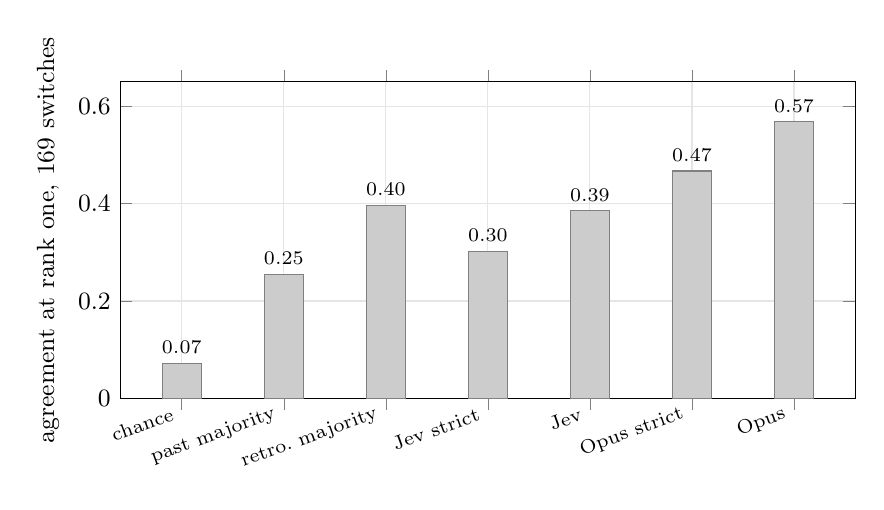
\begin{tikzpicture}
\begin{axis}[
  ybar, bar width=14pt,
  width=0.9\linewidth, height=5.6cm,
  ymin=0, ymax=0.65,
  ylabel={agreement at rank one, 169 switches},
  symbolic x coords={chance, past majority, retro.\ majority, Jev strict, Jev, Opus strict, Opus},
  xtick=data, x tick label style={font=\scriptsize, rotate=20, anchor=east},
  nodes near coords, nodes near coords style={font=\scriptsize, /pgf/number format/fixed, /pgf/number format/precision=2, /pgf/number format/fixed zerofill},
  nodes near coords align={vertical},
  tick label style={font=\small}, label style={font=\small},
  grid=major, grid style={gray!20},
]
\addplot[fill=gray!40, draw=gray] coordinates {(chance,0.072) (past majority,0.254) (retro.\ majority,0.396) (Jev strict,0.302) (Jev,0.385) (Opus strict,0.467) (Opus,0.568)};
\end{axis}
\end{tikzpicture}
\caption{Decomposition at switches. Masking every activity field (``strict'') leaves a residual that depends on the reader: .30 for the small classifier, .47 for Opus~5.5. The unmasked gain over the masked arm (.08 and .10) is what the activity fields add once the sender has changed recipient.}
\label{fig:ladder}
\end{figure}

\paragraph{Cost.}
At list prices the 555 decisions cost \$0.28 with Haiku, \$3.67 with Sonnet and \$7.37 with Opus, about 1.3 cents per decision for the strongest arm against a few hundredths of a cent for the small classifier and nothing for the habit rule. The frontier arms lost 7 rows each to a structured-output grammar limit on candidate sets of 79 or more, in the same direction as the hosted ranker's input cap (11 rows at 66 or more), so every model column is biased toward smaller candidate sets.

\paragraph{What this changes.}
``Mostly habit'' stands as the deployable default: on this stream a free one-line rule beats every model but one, and the one that beats it costs two orders of magnitude more per decision. What changes is the second half of the finding. The ceiling of state-based routing at switches is at least .57, not the small classifier's .39, and about half of the difference survives removing every activity cue. The limiting factor on routing among persistent agents, once a switch is in progress, is how well the state is read, not how much of it there is.

\subsection{From diagnostic to policy}
\label{sec:policy}

The history conditions partition on the label and cannot be observed by a router. The decomposition nonetheless says where a router should be consulted: on switches, which habit gets wrong 71\% of the time when it votes (107 of 150), and on requests with no history, where habit has nothing to say. The deployable question becomes whether anything observable before the decision predicts those rows.

The classifier's own confidence does not separate them (mean top score .65 on continuations, .67 on switches, in live shadow data). Arrival does, partly. Define the trigger ``a candidate with no prior ask participation is present and was active within $T$ seconds''. Evaluated on known switches, the recorded recipient is in the trigger's candidate set on 53.6\% of activations at $T = 600$ (15 of 28); on all worker requests the figure is 27.0\% (20 of 74), and on orchestrator requests 37.5\% (6 of 16). The trigger identifies a set containing the recipient, not a recipient, and its conditional precision is not deployment precision.

Table~\ref{tab:policy} scores the policy ``past majority unless the trigger fires, then choose uniformly among triggered candidates''. With history defined from the full journal it beats past majority at switches (.326 against .254) and on orchestrator switches (.392 against .339) while holding overall agreement. With history defined from the shorter ledger a live router actually sees, everyone looks new, the trigger over-fires, and the policy loses about ten points to habit on continuations. History availability is therefore part of the policy's specification. The threshold was chosen on this data; it is frozen at 600 seconds and the live shadow track has scored it on all traffic since 13 October 2026. The prospective result is the test of this section, and it is not yet available.

\begin{table}[t]
\centering\footnotesize
\caption{Does a diagnostic become a policy? Recipient agreement at rank one. The arrival policy uses past majority unless a never-asked candidate was active within 600 seconds, then chooses uniformly among such candidates.}
\label{tab:policy}
\begin{tabular}{lrrrl}
\toprule
Policy & Worker 555 & Switch 169 & Orch.\ switch 62 & Evidence status \\
\midrule
Past majority & .560 & .254 & .339 & Recorded baseline \\
Jev & .578 & .385 & .371 & Recorded router \\
Opus 5.5 & .775 & .568 & .500 & Recorded router, 70$\times$ cost \\
Arrival policy, journal history & .568 & .326 & .392 & Exploratory replay \\
Arrival policy, ledger history & .511 & .258 & .284 & History-availability sensitivity \\
Arrival policy on later traffic & pending & pending & pending & Prospective, frozen \\
\bottomrule
\end{tabular}
\end{table}

\subsection{A contrast in regime: DecisionBench}
\label{sec:decisionbench}

To check that the arms can rank stateless profile cards at all, and to show what the protocol reports on a dataset with a different history structure, we replayed the aware-c2 condition of DecisionBench \citep{decisionbench2026} (691 delegations). The label is the orchestrator's recorded delegate, not the benchmark's skill annotation, so this is a contrast, not a replication. The classifier on the cards scores .175 at rank one against chance .096, inside the benchmark's published fidelity band, and below an in-order majority of prior delegates (.315), because orchestrators concentrate on a few delegates there too. The history structure is different in kind: 25.6\% of delegations with a previous delegate repeat it, against 66.3\% in the mesh, and the classifier is flat across the same/switch split (.129 against .178). Figure~\ref{fig:mix} is not drawn through DecisionBench because its conditional scores and history definition differ; the point is that the repeat share, with its denominator stated, tells a reader which regime a routing evaluation is in and whether the mix effect can bite.

\section{Related work}

\paragraph{Model routing.}
RouterBench \citep{routerbench2024}, LLMRouterBench \citep{llmrouterbench2026} and TwinRouterBench \citep{twinrouterbench2026} choose which model answers a query or a trajectory step, trading cost against quality. Workers are interchangeable by construction and have no history with the sender. TwinRouterBench's static and dynamic tracks, with router-visible prefixes and execution-verified labels, are the closest methodological relative of our reconstruction; its downstream grounding is exactly what recipient labels do not supply.

\paragraph{Multi-agent construction and delegation.}
MasRouter \citep{masrouter2025} and Uno-Orchestra \citep{unoorchestra2026} build the agent system per task: decomposition, roles, model per role, inference budget. DecisionBench \citep{decisionbench2026} evaluates an orchestrator's choice of delegate from a pool of models with profile cards and finds that fidelity can double while end-task quality stays flat. OrchBench \citep{orchbench2026} evaluates orchestration plans by simulation. We study a different routing object: selecting an already-existing recipient in a changing mesh. We do not claim that no earlier benchmark routes to stateful recipients; we claim that the ones above do not, and that the history structure which makes the mix effect bite is absent from them.

\paragraph{Claimed and attested state.}
The Provenance Paradox \citep{provenance2026} distinguishes self-reported from observed capability and shows self-report can route worse than random. We borrow the vocabulary; because historical descriptions were not journaled, nothing here compares the two.

\paragraph{Repetition baselines and when to override a default.}
Session-based recommendation has long known that a nearest-neighbour or repeat baseline is hard to beat and that evaluation must respect time \citep{sessionrec2018}; temporal link prediction has the same lesson for next-contact prediction \citep{templinkpred2020}; selective prediction formalises choosing when to answer \citep{selectivepred2017}. Our contribution is not those ideas but the measured failure mode and the reporting protocol for persistent-agent routing.

\section{Limitations}

This study measures agreement with recorded recipients in one user's mesh, not optimal recipients or downstream task utility. The registry is reconstructed from activity, descriptions are missing, and selection into the scorable set may favour observable peers; the 75 excluded no-evidence recipients were very likely peers asked at spawn, so the exclusion biases against the no-history findings. Almost all switches belong to one epoch (165 of 169 in May and June); eight occupied weeks are not proven independent, and jointly grouping by week or sender leaves five blocks, one holding 145 requests. The lexical audit removes detected names and project mentions but not indirect identity cues. Thresholds and subgroup analyses are exploratory; model runs are single samples; masks retain activity-selected candidates; the frontier arms required a schema that forbids abstention (Appendix~\ref{app:elicitation}), so their scores are properties of the elicitation as well as the model; hosted model identifiers carry no version, so re-run dates are recorded in place of versions. The DecisionBench adapter differs in history semantics and labels. These boundaries scope the case study; the protocol is reusable without them.

\section{Conclusion}

Among persistent agents most routing decisions repeat the previous one, and an aggregate agreement score rewards that repetition. Conditioning on history turns one number into three, and the three disagree: on this mesh every learned router loses to a one-line rule on continuations and beats it at switches, so the pooled ranking is a property of the request mix. Masking activity shows that the continuation score of every model, including a frontier one, is recency read out of the state; at switches a residual remains whose size is set by the reader, from .30 for a small classifier to .47 for Opus~5.5. The deployable design that follows is a cheap default with a learned override, and the open problem is the trigger, not the ranker. We release the reconstruction, the harness, the history-conditioned metric and a frozen prospective test so that the next persistent-agent router is evaluated on the decisions that need one.

\paragraph{Artifacts.}
\todo{repository URL, data release terms, harness commands.}

\bibliographystyle{plainnat}
\bibliography{refs}

\appendix

\section{Declared divergences from the live tracker}
\label{app:divergences}

Each divergence is listed with its effect on the 169 worker switches. (1)~\emph{Ambiguous reply capture:} an ack with a message can be emitted without a captured reply when delivery fails; 15 historical asks are ambiguous and touch 20 scored switches. Excluding them (149 switches) moves past majority from .254 to .221, newest from .195 to .221, the classifier from .385 to .383 and its strict variant from .302 to .309; no conclusion changes. (2)~\emph{Expiry:} the live tracker evicts lazily; the reconstruction expires at exactly 24 hours. Re-stratifying at 24h10m and 48h changes no scored worker row. (3)~\emph{Forgetting on reaping} is ignored; no scored row changes. (4)~\emph{Self-asks} are counted as inbound but do not set the sender's own last exchange, affecting the sender block of 74 of 1,001 snapshots; masked arms are unaffected. (5)~Daemon restarts wipe the live tracker and are not in the journal, so the reconstruction has fewer no-history rows than a live system would.

\section{Elicitation of the frontier arms}
\label{app:elicitation}

Under a schema that allowed an empty ranking, Opus~5.5 returned no ranking with confidence zero on roughly half of multi-candidate rows; a stricter instruction did not change this (5 of 10 on a fixed probe). Structured outputs reject a minimum array length above one, so the final schema is an object with one required numeric score per candidate key, ranked by score descending with ties in key order, plus a confidence field. On the same probe this yields complete rankings on every row, sharply peaked scores, and 8 of 10 hits. A narrow ``abstained'' outcome (complete answer, confidence exactly zero, all scores equal, at least two candidates) is scored as a miss and does not trip the provider breaker; it occurred once across all three models. The schema fails with a grammar-size error at 79 or more candidates (7 rows per model). Haiku was run with its default reasoning budget and produced 3.5 times the output tokens of the other two models.

\section{Cost of the study}
\label{app:cost}

Small classifier: 6,356 calls, 28.8M input tokens, about \$1.21. Clef Flash: 555 calls, 2.2M input tokens, within a free allocation. Frontier arms: 555 calls each at 1.45M input tokens; output tokens 274k (Haiku), 77k (Sonnet), 79k (Opus); list cost \$0.28, \$3.67, \$7.37, plus \$7.3 for the masked Opus run. DecisionBench replay: about \$0.65.

\end{document}
